\newcommand{\red}{\leq_p}
\newcommand{\problem}[3]{
\begin{definition}
    {#1} \\
    \textbf{Input}: {#2}\\
    \textbf{Output}: {#3}
\end{definition}
}
\newcommand{\bigO}[1]{\mathcal{O}({#1})}

\chapter{Preliminaries}\label{chapter:preliminaries}
In this chapter, we present the background information that supports our work. 
We start with the introduction to the interactive theorem prover Isabelle and its dependencies. 
Furthermore, we present the mathematical backgrounds that are need for verification. 
In the end, we describe the approaches for the complexity analysis and discuss the paradigm 
that is used throughout this work.
\section{Isabelle and Dependencies}
\subsection*{Isabelle/HOL and Archive of Formal Proofs}
Isabelle \cite{wenzel2004isabelle} is a generic interactive theorem prover. HOL is the Isabelle's formalization of Higher-Order Logic, 
a logical system with inductive sets, types , well-founded recursion etc. 
Archive of Formal Proofs \cite{AFP} is a library of verification projects developed by Isabelle. 
Our work is implemented with Isabelle and uses many entries from Archive of Formal 
Proofs.

\subsection*{HOL-Real\_Asymp and Laudau\_Symbols}
HOL-Real\_Asymp is a component of the Isabelle/HOL, in which the asymptotic 
classes are defined. Moreover, the Archive of Formal Proof entry, Landau\_Symbols \cite{Landau_Symbols-AFP}, 
defines the Landau's symbols and provides tool for reasoning about the asymptotic
growth of the functions. 

\subsection*{NREST}
NREST is part of the verification frame work Isabelle-LLVM with time \cite{haslbeck2021verified}. It enables 
the systematic verification of asymptotic complexity of imperative algorithms in Isabelle \cite{zhan2018verifying}. 
We apply this framework 
to verify the polynomial-time complexity of iteration of unordered data structures, such as sets.

\subsection*{The Karp21 Project \cite{polyred}}
The project aims to formalise all of the twenty-one NP-hard problems in Karp's paper in 1972 \cite{karp2010reducibility}. 
Up till now, there are eight problems of them finished, with a few related NP-hard problems that are not in Karp's list. 
Our work also contributes to this project, formalising six of the remaining problems. 
Though dependent on this project, our work only reuses a few existing definitions, 
while the most formalisation and verification is original. An overview of the project is given \hyperref[figure:1]{Figure 2.1}.
The reusable part stems from the reduction from 3CNF-Satisfiabitliy to other problems, for our work starts from Satisfiabitliy.
\begin{oldfigure}[h!]
\centering
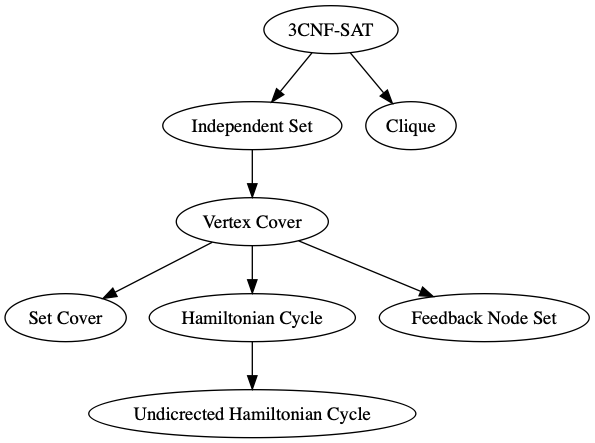
\includegraphics[scale=0.4]{figures/reductions.png}
\caption{The reduction graph of the Karp21 project}
\label{figure:1}
\end{oldfigure}

\subsection*{Positional Notation for Natural Numbers in an Arbitrary Base \cite{DigitsInBase-AFP}}
This entry of Archive of Formal Proofs, short for DigitInBase, shows the uniqueness of representation of natural numbers with an arbitrary base. 
In other words, it proves the well-definedness of the n-ary counting systems. 
Our implementation benefits from this repository in showing the correctness of the polynomial-time reduction from Exact Cover to Subset Sum.

\section{Mathematical Backgrounds}
\subsection*{Asymptotic Notation}
Conventionally, the asymptotic notation is used to define complexity classes and perform the algorithm analysis. 
We follow this convention and choose the big $\mathcal{O}$ notation for algorithm analysis. To begin with, we present a brief
introduction to the asymptotic notation.
\begin{definition}
    Let $f: \mathbb{R} \rightarrow \mathbb{R}$, $g: \mathbb{R} \rightarrow \mathbb{R}$ be two real valued functions. 
    $f(x)$ is big $\mathcal{O}$ of $g(x)$, which writes
    \begin{align*}
        f(x) \in \mathcal{O}(g(x))
    \end{align*}
    if there exists a real $M \geq 0$ and a real $x_0$ s.t. 
    \begin{align*}
        |f(x)| \leq M |g(x)|, \forall x \geq x_0
    \end{align*}
\end{definition}
Thus, $f$ is above bounded by $g$. In other words, $f$ is utmost as complex as $g$. Following this definition, 
we can derive many complexity classes with different $g$. A short list of commonly encountered complexity classes is given 
in \hyperref[table:1]{Table 1}.
\begin{table}[H]
    \centering 
    \begin{tabular}{|| c | c | c ||}
        \hline 
        Name & Big $\mathcal{O}$ Notation & Algorithmic Examples \\ 
        \hline 
        Constant & $\mathcal{O}(1)$ & Parity check\\
        \hline 
        Logarithmic & $\mathcal{O}(\log n)$ & Binary search in a sorted array \\ 
        \hline 
        Linear & $\mathcal{O}(n)$ & Addition of integers \\
        \hline 
        Quasilinear & $\mathcal{O}(n\log n)$ & Merge-sort and heap-sort \\
        \hline 
        Polynomial & $\mathcal{O} (n^c), c \in \mathbb{N}$ & Matrix multiplication \\
        \hline 
        Factorial & $\mathcal{O} (n!)$ & Enumeration of partitions of a set\\
        \hline 
    \end{tabular}
    \caption{List of commonly encountered complexity classes.}
    \label{table:1}
\end{table}

In this work, we only consider the polynomial class. For simplicity, we did not 
formalise the theory of asymptotic classes and big $\mathcal{O}$ notation but used the 
available \textsc{Isabelle} dependencies of \textbf{HOL-Real\_Asymp} and \textbf{Landau\_Symbols}.

\subsection*{Decision Problems}
\begin{definition}
    A decision problem is a yes-no question on an infinite set of fixed type of inputs.
\end{definition}
Generally, if we refer to a decision problem $A$, we refer to the set of inputs whose answer to the yes-no question is yes. 
We follow this convention throughout this work.
The handling of a decision problem usually involves two questions:
\begin{enumerate}
    \item Is there a terminating algorithm which computes the solution to this problem?
    \item If the answer to the first question is yes, is this algorithm efficient?
\end{enumerate}
If the answer to the first question is yes for a problem, it is a decidable problem, otherwise it is non-decidable. 
We do not expect a yes-no answer for the second question, but would like to find 
the optimal complexity for the algorithm, e.g. logarithmic complexity, polynomial complexity, etc. 
While some problems are possible to be computed in an optimal complexity by a deterministic algorithm, 
there are also a few problems, for which no deterministic polynomial-time algorithm is found. 
We limit these problems and given them a formal definition.
\begin{definition}
    If there is a deterministic algorithm that decides the solution 
    to the problem in polynomial time, the problem is in the complexity class \textbf{P}.
    If this polynomial algorithm is non-deterministic, the problem is in the complexity class \textbf{NP}. 
\end{definition}
\begin{definition}
If a problem is at least as complex as the most complex problems in \NP. It is 
    in the complexity class \textbf{NP-hard}.
\end{definition}

Instead of trying to prove or reject the existence of a non-deterministic algorithm 
for the NP problems, we focus on the NP-hardness. We would like to formally prove 
that many classical decision problems are NP-hard. For this reason, we have to introduce polynomial-time reductions.

\subsection*{Polynomial-time Reductions}
\begin{definition}
    Given two decision problems $A$ and $B$, 
a reduction is a function $f: A \rightarrow B$, 
which maps the instances of $A$ to those of $B$. A reduction is a polynomial-time reduction
if and only if the reduction function has a polynomial-time complexity. 
For a polynomial-time reduction from $A$ to $B$, we write $A \red B$. 
\end{definition}
Let $M$ and $N$ denote the universe of $A$ and $B$. 
A function $g: M \rightarrow N$ is a polynomial-time reduction 
if and only if the following conditions are satisfied.
\begin{align*}  
    &x \in A \iff g(x) \in B \\
    &\exists k\in \mathbb{N}. g \in \mathcal{O}(n^k)
\end{align*}
For convenience, we separate (2.1) into the soundness and completeness of the reduction.
\begin{align*}
    soundness: \quad x \in A \Longrightarrow g(x) \in B \\
    completeness: \quad g(x) \in B \Longrightarrow x \in A
\end{align*}

\subsection*{Satisfiability}
To show a decision problem $B$ is NP-hard, 
we have to find a NP-hard problem $A$ and polynomial-time reduction 
such that $A \red B$. The first proven NP-hard problem is Satisfiability, 
which was independently proven by Cook in 1971 \cite{cook2023complexity} and Levin in 1973 \cite{levin1973universal}. 
The Satisfiability problem is defined by 
\problem{Satisfiability}{A propositional logical formula in 
conjunctive normal form. }{Is there a valid assignment for this formula?}
In the previous implementation of the project, Satisfiability is defined by a list of clauses, with the clauses as sets of variables.
Our first reduction also stems from Satisfiability, while all the other reductions are constructed upon novel introduced problems. 
More details on the reduction and implementation are given in \hyperref[chapter:covering]{Chapter 3} and \hyperref[chapter:weighted]{Chapter 4}. 
A glimpse of the available definition is given by \hyperref[figure:2]{Figure 2.2}. \\\\
In this definition, a literal is defined as either a positive or negative existence of the variables. Then 
the type \textbf{three\_sat} is defined. It is technically not a 3-Satisfiability instance, for each clause can 
contain more than three literals. This naming mistake is a historical legacy, which should be renamed after negotiation with the original contributors.
After this, the definitions of \textbf{lifting}, \textbf{models}, and \textbf{sat} are given. They describe how an assignment is checked over the propositional 
logical formula. Finally, we add the definition of \textbf{cnf\_sat}, upon which our first reduction is defined.
\begin{figure}[!h]
    \Snippet{cnf-sat-def}
    \caption{Definition of Satisfiability}
    \label{figure:2}
\end{figure}

\section{Application of NREST and Paradigms}
The NREST package offers an approach for approximating the complexity of non-deterministic processes.
This is especially useful when iterating a set, a collection or any other unordered data structures. Thus,
we use this package throughout this work. In our complexity analysis, the following commands are used. 
\begin{itemize}
    \item \textbf{$RETURNT$ res}. A command that returns the result \textbf{res}. It costs exactly one unit of time.
    \item \textbf{$SPECT$ [cond $\rightarrow$ cost]}. A command used for checking a condition. Checking the condition \textbf{cond}
    take \textbf{cost} units of time.
    \item \textbf{$SPEC$ $P$ $Q$}. A command used for assignment. 
    Should $P\ x$ hold for an object $x$, it is a valid object after the assignment.
    This assignment takes $Q\ x$ units of time.
\end{itemize}
To apply the NREST approach in the complexity analysis, it is necessary to rewrite the algorithm with the NREST commands.
In our implementation, it means to convert the reduction function into an algorithm implemented with NREST commands.
During the conversion, we follow the following principles for complexity analysis.
\begin{enumerate}
    \label{para1}
    \item Checking the condition always costs exactly one unit of time. 
    \item During the iteration, it costs one unit of time each for access, modification and insertion of the set elements.
    \item All other operations should cost one unit of time, if not stated explicitly.
\end{enumerate}
Then, it is possible show the property of the reduction with this approach. In addition to the polynomial-time complexity, 
the existing definition of polynomial-time reduction in the Karp21 project requires a polynomial-space complexity, too. 
We are consistent with this definition, and hence verified the polynomial-space complexity in each reduction as well.
Let $f$ denote a polynomial-time reduction from $A$ to $B$, while $f_{alg}$ denotes the NREST version of the reduction.
Furthermore, we define sizing functions $s_A$ and $s_B$ as metrics for the asymptotic classes.
To show that the reduction is polynomial, we show that the reduction is polynomial bounded in terms 
of time and space, which are respectively the \textit{refines} and the \textit{size} lemma.
\begin{align*}
    refines: \quad f_{alg}(A) \leq \mathcal{O}((s_A(A))^k) \\
    size: \quad s_B (f(A)) \leq \mathcal{O}((s_A(A))^k)
\end{align*}
In the end, we can conclude the following implementation paradigm to show that a reduction is correct and polynomial.
\begin{enumerate}
    \item Implement the reduction in Isabelle/HOL.
    \item Prove that the reduction is correct.
    \item Implement the reduction in NREST commands.
    \item Prove that the reduction costs polynomial time.
    \item Prove that the algorithm costs polynomial space.
\end{enumerate}
